\section{Results}
\label{sec:results}

In this section we present the main results of this work,
namely the
determination of the photon PDF $x\gamma(x,Q)$ from a fit to 
HERA inclusive structure functions and ATLAS high-mass Drell-Yan cross sections.
%
First of all,
we assess the fit quality and compare the fit results
with the experimental data.
%
Then, the resulting photon PDF is shown and compared with other
recent determinations.
%
Here the impact of the high mass DY data on
the quark and gluon PDFs is also quantified.
%
Following this,
the robustness of the fits of $x\gamma(x,Q)$
with respect to varying the model, parametrization, and procedural
inputs is assessed.
%
Finally, perturbative stability is addressed by comparing NLO and
NNLO results.

\subsection{Fit quality and comparison between data and fit results}

In the following, the results that will be shown
correspond to those obtained from fitting the
double-differential $\lp m_{ll},y_{ll}\rp$ distributions.
%
We have verified that comparable results are obtained if the
$\lp m_{ll},\Delta\eta_{ll}\rp$ distributions are fitted instead.

Using the NNLO fit settings discussed in Sect.~\ref{sec:fitsettings},
a $\chi^{2}/N_{\rm dof} = 1236/1056$ is obtained
for the HERA inclusive data, and a partial
$\chi^2/N_{\rm data} = 48/48$ for the high-mass Drell-Yan data,
where $N_{\rm dof}$ is the number of degree of freedom in the fit and 
$N_{\rm data}$  is the number of data points for the ATLAS data.
%
These values for  $\chi^{2}/N_{\rm dat}$, together
with the corresponding values for the various
invariant mass $m_{ll}$ bins of the ATLAS  data,
are summarised in
Table~\ref{tab:chi2fit}.
%
The quality of the agreement with the HERA inclusive structure
functions is of comparable quality to that found in the HERAPDF2.0 analysis.
%
Note that in the calculation of the total $\chi^2$ for the
ATLAS data, the correlations between the
different $m_{ll}$ bins have been taken into account.

%%%%%%%%%%%%%%%%%%%%%%%%%%%%%%%%%%%%%%%%%%%%
\begin{table}[t]
  \centering
  \begin{tabular}{|c|c|}
    \hline
    Dataset  &   $\chi^2$ \\
    \hline
    \hline
    HERA I+II & 1236/1056\\
    \hline
    HMDY  116 GeV $\ge m_{ll} \ge $ 150 GeV  &  9/12 \\
    HMDY  150 GeV $\ge m_{ll} \ge $ 200 GeV  &  15/12 \\
    HMDY  200 GeV $\ge m_{ll} \ge $ 300 GeV  &  14/12 \\
    HMDY  300 GeV $\ge m_{ll} \ge $ 500 GeV  &  5/6 \\
    HMDY  500 GeV $\ge m_{ll} \ge $ 1500 GeV &  4/6 \\
    \hline
    Correlated (HMDY) $\chi^2$ & 1.17 \\
    Log penalty (HMDY) $\chi^2$  & -0.12 \\
    \hline
    \hline
    Total  (HMDY) & 48/48 \\
    \hline
    \end{tabular}
  \caption{The $\chi^{2}/N_{\rm dat}$ in the NNLO fits for the
    HERA inclusive structure functions and for the various
    invariant mass $m_{ll}$ bins of the ATLAS high-mass DY data.
        %
    In the latter case, we also indicate the contribution to the
    $\chi^2$ which arises from the correlated and log-penalty terms.
\label{tab:chi2fit}
  }
\end{table}
%%%%%%%%%%%%%%%%%%%%%%%%%%%%%%%%%%%

Figs.~\ref{hmDY_2D_1}--\ref{hmDY_2D_3} then show the
comparison between the results of the NNLO fit, in the following
denoted by {\tt xFitter\_epHMDY},
and the ATLAS data
  for the $(m_{ll},|y_{ll}|)$ double-differential Drell-Yan cross-sections
  as function of $|y_{ll}|$, for the five bins in $m_{ll}$ separately.
  %
  The comparisons are shown both
  in an absolute scale  and as ratios to the central value
  of the experimental data.
  %
  The error bars on the data points correspond to the statistical
  uncertainties, while the yellow bands
  indicate instead to size of the correlated systematic uncertainties.
  %
  The solid lines indicate the theory calculations obtained using the results
  of the fit, with the dashed lines including as well the systematic shifts.
  %
  In the lower panels of ratio plots,
  we show the $\chi^2$ pulls between fit and data for each $y_{ll}$ bin,
  defined as the different between data and theory in units
  of the total experimental uncertainty.


%%%%%%%%%%%%%%%%%%%%%%%%%%%%%%
\begin{figure}[t]
\centering
\includegraphics[width=14cm]{figs/data_401-1.pdf}\\
\includegraphics[width=14cm]{figs/data_402-1.pdf}
\caption{Comparison between the results of the fit and the ATLAS data
  for the $(m_{ll},|y_{ll}|)$ double-differential Drell-Yan cross-sections
  as function of $|y_{ll}|$, for the first two $m_{ll}$ bins.
  %
  The comparisons are shown both
  in an absolute scale (left plots) and as ratios to the central value
  of the experimental data (right plots).
  %
  The error bars on the data points correspond to the statistical
  uncertainties, while the yellow bands
  indicate instead to size of the correlated systematic uncertainties.
  %
  The solid lines indicate the theory calculations obtained using the results
  of the fit {\tt xFitter\_epHMDY}, with the dashed lines including as well the systematic shifts.
  %
  In the lower panels of ratio plots, we show the $\chi^2$ pulls between fit and data for each $y_{ll}$
  bin.
}
\label{hmDY_2D_1}
\end{figure}

%%%%%%%%%%%%%%%%%%%%%%%%%%%%%%
\begin{figure}[t]
\centering
\includegraphics[width=14cm]{figs/data_403-1.pdf}\\
\includegraphics[width=14cm]{figs/data_404-1.pdf}
\caption{Same as Fig.~\ref{hmDY_2D_1} for the third and fourth $m_{ll}$ bins.
}
\label{hmDY_2D_2}
\end{figure}

%%%%%%%%%%%%%%%%%%%%%%%%%%%%%%
\begin{figure}[t]
\centering
\includegraphics[width=14cm]{figs/data_405-1.pdf}
\caption{Same as Fig.~\ref{hmDY_2D_1} for the highest $m_{ll}$ bins.
}
\label{hmDY_2D_3}
\end{figure}
%%%%%%%%%%%%%%%%%%%%%%%%%%%%%%%

As can be seen from Fig.~\ref{hmDY_2D_1}--\ref{hmDY_2D_3}, there
is good agreement between ATLAS data and the NNLO theory
predictions obtained from the {\tt xFitter\_epHMDY} fit.
%
This agreement is consistent with the values of the $\chi^2$ reported in
Table~\ref{tab:chi2fit}, where for the ATLAS data we found
that $\chi^2/N_{\rm dat}=1$, and is particularly remarkable
given the high precision of the data, with total experimental
uncertainties at the few percent level in most of the kinematic range.

\subsection{The photon PDF from LHC high-mass DY data}

We now present the results of the {\tt xFitter\_epHMDY}
fit of the photon PDF $x\gamma$ and compare with
other recent determinations. We will also assess the impact
of the ATLAS high-mass DY data on the quark and gluon PDFs as compared
to a fit with only HERA structure functions as input.

%%%%%%%%%%%%%%%%%%%%%%%%%%%%%%%%%%%%%%%%%%%%%%%%%%%%%%%%
\begin{figure}[t]
  \includegraphics[width=7cm]{figs/photon_comp_10000.pdf}
  \includegraphics[width=7cm]{figs/photon_comp_10000_ratio.pdf} 
  \caption{Left plot: comparison between the photon $x\gamma(x,Q^2)$ at $Q^2=10^4$ GeV$^2$
    from the present NNLO analysis ({\tt xFitter\_epHMDY}) with the
    corresponding results from NNPDF3.0QED, LUXqed and HKR16.
  %
  Right plot: the same comparison, now with the results normalized to the central value
  of {\tt xFitter\_epHMDY}.
  %
  For the present fit, we show the PDF uncertainties at the 68\% CL obtained from the MC method,
  while model and parametrization uncertainties are discussed below.
  %
  For HKR16 only the central value is shown, while for LUXqed we include
  the associated PDF uncertainty band~\cite{Manohar:2016nzj}. }
\label{photon_zoom} \label{photon_zoom_ratio}
\end{figure}
%%%%%%%%%%%%%%%%%%%%%%%%%%%%%%%%%%%%%%%%%%%%%%%%%%%%%%%%

In Fig.~\ref{photon_zoom}, the photon PDF $x\gamma(x,Q)$ is shown at
$Q^2=10^4$ GeV$^2$,  and compared to the corresponding LUXqed,
HKR16 and NNPDF3.0QED results.
%
In the left plot we comparison is presented in an absolute scale, while
in the right plot we show the ratio of
different results normalized to
the central value of our fit.
%
For the present fit, {\tt xFitter\_epHMDY}, we show here
the experimental PDF uncertainties at the 68\% confidence level (CL) obtained from the Monte Carlo method,
 while model and parametrization uncertainties are discussed below.
 %
Likewise, for NNPDF3.0QED we show the 68\% CL uncertainty band.
 %
For HKR16, only the central value is available, while for LUXqed we include
the associated PDF uncertainty band computed according to the
prescription of Ref.~\cite{Manohar:2016nzj}.
%
The $x$-range in Fig.~\ref{photon_zoom} has been restricted to the region
$0.02 \le x \le 0.9$, since beyond that region the ATLAS
data has very limited sensitivity to $x\gamma$.

From Fig.~\ref{photon_zoom} we find that for $x\ge 0.1$ the four determinations of
the photon PDF which are being compared here are consistent within PDF uncertainties.
%
For smaller values of $x$, the photon PDF from LUXqed and HKR16 is somewhat smaller than {\tt xFitter\_epHMDY},
but still in agreement at the 2-$\sigma$ level.
%
As we will show below, this agreement is further improved if the PDF uncertainties in
{\tt xFitter\_epHMDY}
arising from variations of the input parametrization are added to the experimental
uncertainties.
%
Moreover, the results of this work and NNPDF3.0QED agree at the 68\% CL for $x\ge 0.03$,
and agreement which extends to smaller values of $x$ once the parametrization
uncertainties in {\tt xFitter\_epHMDY} are accounted for.
%
Across the entire range of $x$, the LUXqed and the HKR16 calculations of $x\gamma$ are very close
to each other.

Concerning the size of the uncertainties, from Fig.~\ref{photon_zoom} we see that,
for $0.04 \le x \le 0.2$, the present analysis  exhibits smaller PDF
uncertainties as compared to those from  NNPDF3.0QED.
%
Indeed, the experimental uncertainty on the present fit
turns out to be at the  $\sim 30\%$ level for $x\le 0.1$, from where it increases
rapidly specially in the positive direction, since variations of $x\gamma$ in the negative
direction are constrained by positivity.
%
On the other hand, we also find that the limited sensitivity of the ATLAS data to the photon
PDF does not allow to obtain a determination with uncertainties
competitive with those of LUXqed.

It is interesting to also assess the impact of the high-mass Drell-Yan 8 TeV measurements on
the light quark and gluon PDFs.
%
For this purpose, and since HERA inclusive data alone (which should be used as
benchmark for this comparison) does not have sensitivity to the photon
PDF, the fits have been repeated freezing the photon PDF to the
{\tt xFitter\_epHMDY} shape.
%
This way, a 
a meaningful comparison between the HERA-only
baseline and the HERA+HMDY fit can be performed, to gauge the modifications of quark and
gluon PDFs.
%
This comparison is shown in Fig.~\ref{fig:QCDfit} for the up and down
antiquarks, for which the effect of the high-mass Drell-Yan data is
expected to be most pronounced. PDFs are presented as ratios to the
central value of the HERA+HMDY fit with their experimental uncertainties.
%
As is apparent from this comparison, the modifications in the medium
and large-$x$ antiquark distributions from the HMDY data are
significant for $x\ge 0.01$, although the two fits agree always at the
one-sigma level.
%
The improvement of the PDF
uncertainties is particularly marked for the case of $x\bar{d}$,
%
These results were cross-checked with fits obtained by switching
off the QED effects for both HERA only fits and the nominal fits, with
the same outcome.

%%%%%%%%%%%%%%%%%%%%%%%%%%%%%%
\begin{figure}[t]
\centering
\includegraphics[width=7cm]{figs/q2_7_5_pdf_ubar_ratio.pdf}
\includegraphics[width=7cm]{figs/q2_7_5_pdf_dbar_ratio.pdf} 
\caption{The impact of the ATLAS high-mass 8 TeV Drell-Yan measurements
  on the $x\bar{u}$ and $x\bar{d}$ sea quark PDFs at the input
  parametrization scale $Q^2=7.5$ GeV$^2$.
  %
  The results are shown normalized to the central value of {\tt xFitter\_epHMDY}. 
  }
\label{fig:QCDfit}
\end{figure}
%%%%%%%%%%%%%%%%%%%%%%%%%%%%%%%


Following this presentation of the main features of the {\tt
  xFitter\_epHMDY} analysis, the stability of the fit and its robustness
to model, parametrization, and procedural uncertainties are assessed.

\subsection{Robustness and perturbative stability checks}
\label{sec:crosschecks}

In this section the robustness of our determination of the
photon PDF $x\gamma(x,Q)$ is assessed with respect to a number of variations.
Firstly variations of the values of
physical parameters, like $\alpha_s$ or the charm mass are explored, secondly
variations of the choices made for the PDF parametrization, and thirdly 
variations associated to different fitting procedures.
%
One variation at a time is explored and its effect on the
central value of the photon PDF is compared with the size of the experimental
uncertainty computed using the Monte-Carlo method.

Firstly, the impact of uncertainties associated to either
the choice of some physical parameters or of some specific settings
adopted in the fit are explored.
%
Fig.~\ref{fig:model} shows the comparison between the baseline
determination of $x\gamma(x,Q)$ at $Q^2=10^4$ GeV$^2$ in the present
analysis (including the experimental uncertainties) with the central
value of those fits for which a number of variations have been
performed.
%
In particular, we have considered the following variations:
\begin{itemize}
\item The strong coupling constant is varied by $\delta \alpha_s=\pm 0.002$ around the central value.
\item The ratio of strangeness to non-strange PDFs is decreased to $r_s=0.75$ instead of $r_s=1$.
\item The value of the charm mass is varied between $m_c=1.41$ GeV and $m_c=1.53$ GeV,
  and that of the bottom mass between $m_b=4.25$ GeV and $m_b=4.75$ GeV.
\item The minimum value $Q_{\rm cut}$ of the fitted data is decreased down to $\sqrt{5}$ GeV.
\item The parametrization scale $Q_0$ is raised to $\sqrt{10}$ GeV as compared
  to the baseline value of $Q_0=\sqrt{7.5}~$GeV.
\end{itemize}
The results of Fig.~\ref{fig:model} show that in all cases the effect
of all the variations is contained within (and typically much smaller than) 
the experimental PDF uncertainty bands of the reference fit.

%%%%%%%%%%%%%%%%%%%%%%%%%%%%%%                                          
\begin{figure}[t]
\centering
\includegraphics[width=7cm]{figs/q2_10000_pdf_ph_model_1}
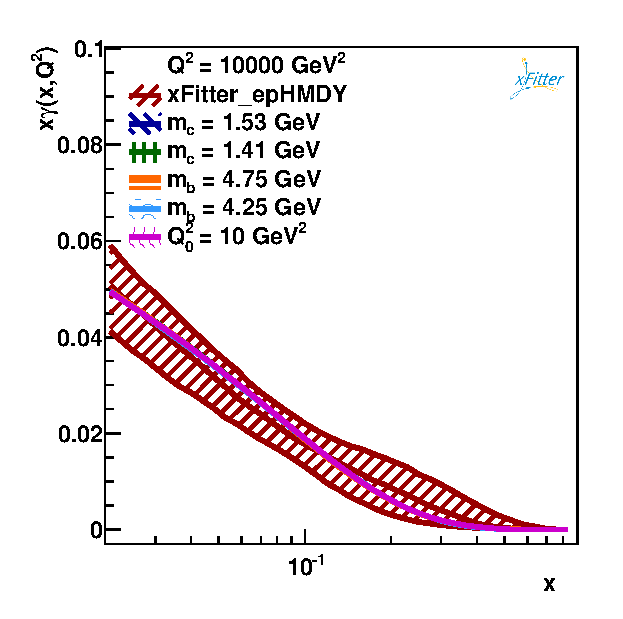
\includegraphics[width=7cm]{figs/q2_10000_pdf_ph_model_2}
\caption{Comparison between the baseline determination of
  $x\gamma(x,Q^2)$ at $Q^2=10^4$ GeV$^2$ in the present
  analysis, {\tt xFitter\_epHMDY},
  with the central value of a number of fits for which one input parameter has been varied.
  %
  The following variations have been considered: $r_s=0.75$, $Q^2_{\rm cut}=5$ GeV$^2$, $\alpha_s=0.116$ and
  0.118 (left plot); and
  $m_c=1.41$ and 1.53 GeV, $m_b=4.25$ and 4.75 GeV, and $Q_0^2=10$ GeV$^2$ (right plot).
  %
  See text for more details about these variations.
}
\label{fig:model}
\end{figure}
%%%%%%%%%%%%%%%%%%%%%%%%%%%%%%

Another important check of the robustness of the present determination of
$x\gamma$ can be obtained by comparing the baseline fit with further
fits where a number of new free parameters are allowed in the PDF
parametrization, in addition to those listed in Eq.~(\ref{eq:param}).
%
Fig.~\ref{fig:param} shows the impact of three representative
variations (others have been explored, leading to smaller
differences): more flexibility to the gluon distribution, allowing it
to become negative at the initial scale (labeled by ${\rm neg}$), adding on top $D_{u_v}$,
and then $D_{\bar{u}}+D_{\bar{d}}$.
%
As before, all variations are contained within the MC PDF uncertainty
bands, though the impact of the parametrization variations is larger
than that of the model variations: in the case of the
${\rm nefg}+D_{\bar{u}}+D_{\bar{d}}$ variations, the central value is
at the edge of the lower uncertainty band.
%
Importantly, once this additional uncertainty coming from the
parametrization variations is accounted for, the agreement of the present fit
with LUXqed and HKR16 improves in the region around $x\simeq 0.02$.

An important cross-check of the robustness of the estimated
uncertainty of the photon PDF in this analysis is provided by the
comparison of the Monte-Carlo method with the Hessian method.
%
In Fig.~\ref{fig:photon_mc_vs_hessian} we show this comparison, which
indicates a reasonable agreement between the two methods.
%
In particular, the central values of the photon obtained with the two
fitting techniques are quite similar to each other.

%%%%%%%%%%%%%%%%%%%%%%%%%%%%%%%%%%%
\begin{figure}[t]
\centering
\includegraphics[width=7cm]{figs/q2_10000_pdf_ph_param_var.pdf}
\includegraphics[width=7cm]{figs/photon_mc_vs_hessian} 
\caption{Left: the impact on the photon PDF $x\gamma(x,Q^2)$
  from {\tt xFitter\_epHMDY}
  in fits where a number of additional free parameters are allowed
  in the PDF parametrization Eq.~(\ref{eq:param}).
  %
  The parametrization variations that have been explored
  are: more flexibility to the gluon distribution, allowing
  it to become negative
  (labeled by ``${\rm neg}$''), adding on top $D_{u_v}$, and then
  adding $D_{\bar{u}}+D_{\bar{d}}$.
 %
 Right: comparison between the {\tt xFitter\_epHMDY} determinations obtained with the
 Monte Carlo (default) and with the Hessian methods, where in
  both cases the PDF error band  shown corresponds to the 68\% CL uncertainties.  }
\label{fig:param}
\label{fig:photon_mc_vs_hessian}
\end{figure}
%%%%%%%%%%%%%%%%%%%%%%%%%%

To complete this section, an interesting exercise is to quantify the perturbative stability of
the present fit of the photon PDF $x\gamma(x,Q)$ with respect to the inclusion
of NNLO QCD corrections in the analysis.
%
To study this, Fig.~\ref{fig:nlo_vs_nnlo} shows a
comparison between the baseline fit of $x\gamma(x,Q)$, based on NNLO
QCD + NLO QED theory, with the central value resulting from a fit
based instead on NLO QCD theory (with the QED part identical in both
cases).
%
For the NNLO fit, only the experimental PDF uncertainties, estimated
using the Monte-Carlo method, are shown.

From the comparison of Fig.~\ref{fig:nlo_vs_nnlo}, it is clear that the
fit of $x\gamma(x,Q)$ exhibits a reasonable perturbative stability,
since the central value of the NLO fit is always contained in the
one-sigma PDF uncertainty band of the baseline determination based on
NNLO QCD + NLO QED.
%
The agreement between the two fits is particularly good for
$x\gsim 0.1$, where the two central values are very close to each
other.

%%%%%%%%%%%%%%%%%%%%%%%%%%%%%%%%%%%%%%%%%%%%%%%%%%%%%%%%%%%%%%%%%%%%%%%%%%%%%%%%%%%%%%%%%%%%%
%%%%%%%%%%%%%%%%%%%%%%%%%%%%%%%%%%%%%%%%%%%%%%%%%%%%%%%%%%%%%%%%%%%%%%%%%%%%%%%%%%%%%%%%%%%%%
\begin{figure}[t]
\centering
\includegraphics[width=7cm]{figs/q2_7_5_pdf_ph_NLOvsNNLO.pdf}
\includegraphics[width=7cm]{figs/q2_10000_pdf_ph_NLOvsNNLO.pdf}
\caption{Left plot: comparison between the reference {\tt xFitter\_epHMDY}
  fit of $x\gamma(x,Q^2)$, based on  NNLO QCD and NLO QED theoretical
  calculations, with the central value of the corresponding fit based
  on NLO QCD and QED theory, at $Q^2=7.5$ GeV$^2$.
  %
  In the former case, only the experimental Monte Carlo PDF
  uncertainties are shown.
  %
  Right plot: same comparison, now presented at the higher scale of $Q^2=10^4$ GeV$^2$.  }
\label{fig:nlo_vs_nnlo}
\end{figure}
%%%%%%%%%%%%%%%%%%%%%%%%%%%%%%%%%%%%%%%%%%%%%%%%%%%%%%%%%%%%%%%%%%%%%%%%%%%%%%%%%%%%%%%%%%%%
%%%%%%%%%%%%%%%%%%%%%%%%%%%%%%%%%%%%%%%%%%%%%%%%%%%%%%%%%%%%%%%%%%%%%%%%%%%%%%%%%%%%%%%%%%%%
